\documentclass[aspectratio=169,11pt]{beamer}

\usepackage[T1]{fontenc}
\usepackage[sfdefault]{sourcesanspro}
\usepackage{sfmath}
\usepackage{amsmath,amssymb}
\usepackage{booktabs,tabularx,array,colortbl}
\usepackage{pgfplots}
\usepackage{microtype}
\usepackage{xurl}

\pgfplotsset{compat=1.18}

% -----------------------------------------------------------------------------
% Visual system
% -----------------------------------------------------------------------------
\definecolor{Navy}{HTML}{18324B}
\definecolor{Teal}{HTML}{138A8A}
\definecolor{Orange}{HTML}{E07A45}
\definecolor{Gold}{HTML}{CAA032}
\definecolor{WarmWhite}{HTML}{F7F4EE}
\definecolor{PaleTeal}{HTML}{E4F0EF}
\definecolor{PaleOrange}{HTML}{F8E9E0}
\definecolor{MidGray}{HTML}{65717C}
\definecolor{LightGray}{HTML}{D8DEE3}

\setbeamertemplate{navigation symbols}{}
\setbeamertemplate{itemize item}{\color{Teal}\raise0.15ex\hbox{\rule{0.55ex}{0.55ex}}}
\setbeamertemplate{itemize subitem}{\color{Teal}\raise0.15ex\hbox{\rule{0.40ex}{0.40ex}}}
\setbeamersize{text margin left=9mm,text margin right=9mm}

\setbeamercolor{normal text}{fg=Navy,bg=WarmWhite}
\setbeamercolor{frametitle}{fg=Navy,bg=WarmWhite}
\setbeamercolor{footline}{fg=MidGray,bg=WarmWhite}
\setbeamercolor{structure}{fg=Teal}
\setbeamerfont{normal text}{size=\fontsize{16.2}{20}\selectfont}
\setbeamerfont{frametitle}{size=\fontsize{25}{28}\selectfont,series=\bfseries}
\setbeamerfont{footline}{size=\fontsize{7.8}{9}\selectfont}

\setbeamertemplate{frametitle}{%
  \vspace{2.5mm}%
  \insertframetitle\par
  \vspace{1.4mm}%
  {\color{Teal}\rule{19mm}{1.5pt}}%
}

\setbeamertemplate{footline}{%
  \leavevmode%
  \hbox{%
    \begin{beamercolorbox}[wd=.82\paperwidth,ht=3.0ex,dp=1.25ex,leftskip=9mm]{footline}%
      Block-adaptive Bayesian local projections \hspace{0.9em} Current state: 8 September 2026
    \end{beamercolorbox}%
    \begin{beamercolorbox}[wd=.18\paperwidth,ht=3.0ex,dp=1.25ex,rightskip=9mm plus 1fil]{footline}%
      \insertframenumber\,/\,9
    \end{beamercolorbox}%
  }%
}

\newcommand{\keypoint}[1]{\textcolor{Teal}{\textbf{#1}}}
\newcommand{\warning}[1]{\textcolor{Orange}{\textbf{#1}}}
\newcommand{\smallsource}[1]{%
  \par\vfill{\fontsize{8.6}{10.2}\selectfont\color{MidGray}#1}%
}
\newcommand{\statusrow}[3]{%
  \textcolor{#1}{\bfseries #2} & #3\\[2.3mm]
}

\begin{document}

% -----------------------------------------------------------------------------
% 1. Cover
% -----------------------------------------------------------------------------
{
\setbeamercolor{background canvas}{bg=Navy}
\begin{frame}[plain]
  \color{WarmWhite}
  \vspace{8mm}
  {\color{Teal}\rule{22mm}{2.6pt}}\par
  \vspace{7mm}
  {\fontsize{36}{41}\selectfont\bfseries
    Where does the VAR prior fail?\par}
  \vspace{4mm}
  {\fontsize{22}{27}\selectfont
    Block-adaptive Bayesian local projections\par
    under sparse dynamic misspecification}
  \vfill
  {\fontsize{15}{19}\selectfont\color{LightGray}
    MSc thesis project\par
    Stefano Graziosi\par
    8 September 2026}
  \vspace{5mm}
  {\fontsize{12}{15}\selectfont\color{LightGray}
    Status: methodological prototype and Monte Carlo evidence. No empirical results yet.}
\end{frame}
}

% -----------------------------------------------------------------------------
% 2. Motivation
% -----------------------------------------------------------------------------
\begin{frame}{The research question}
  \vspace{-1mm}
  \begin{columns}[T,onlytextwidth]
    \column{0.47\textwidth}
      {\fontsize{19}{22}\selectfont\color{Teal}\bfseries Local projections}\par
      \vspace{2mm}
      Estimate each horizon directly. They tolerate richer dynamics, but
      impulse responses can be imprecise in modest samples.

    \column{0.06\textwidth}
      \centering
      \vspace{10mm}
      {\color{LightGray}\rule{0.7pt}{25mm}}

    \column{0.47\textwidth}
      {\fontsize{19}{22}\selectfont\color{Orange}\bfseries VARs}\par
      \vspace{2mm}
      Impose one dynamic system across horizons. They gain precision when
      that system is adequate, but transmit misspecification everywhere.
  \end{columns}

  \vspace{5mm}
  {\fontsize{14.3}{18}\selectfont\color{MidGray}
    A global Bayesian LP compromises by shrinking every coefficient block
    toward a VAR-implied centre with the same horizon-specific tightness
    $\lambda_h$.}

  \vspace{5mm}
  \colorbox{PaleTeal}{%
    \parbox{0.955\textwidth}{%
      \vspace{2.2mm}
      {\fontsize{20}{24}\selectfont\bfseries
       When the VAR is wrong in one part of the system, can only that part
       of the LP escape the prior?}
      \vspace{2.2mm}
    }%
  }
\end{frame}

% -----------------------------------------------------------------------------
% 3. Method
% -----------------------------------------------------------------------------
\begin{frame}{Block-adaptive VAR-centred shrinkage}
  \vspace{-2mm}
  {\fontsize{17}{21}\selectfont
  \begin{align*}
    y_{i,t+h} &= z_t'\beta_{i,h}+u_{i,t+h},\\[-1mm]
    \beta_{i,g,h}-\mu^{\mathrm{BVAR}}_{i,g,h}
      &\sim \mathcal N\!\left(
        0,\ \sigma^2_{i,h}\lambda_h^2\tau_{i,g,h}^2D_{g,h}
      \right),
      & \tau_{i,g,h}&\sim\mathcal C^+(0,1).
  \end{align*}}

  \vspace{-2mm}
  \begin{columns}[T,onlytextwidth]
    \column{0.64\textwidth}
      {\fontsize{14.5}{18}\selectfont
      In each response equation and horizon, one block collects all $p$
      coefficients attached to the lags of predictor variable $g$.

      \vspace{4mm}
      \[
      \beta_{i,h}=\Bigl[
        \alpha_{i,h}\ \Big|\
        \underbrace{\boldsymbol\beta_{i,1,h}}_{\color{Teal}\text{lags of }y_1}\ \Big|\
        \underbrace{\boldsymbol\beta_{i,2,h}}_{\color{Orange}\text{lags of }y_2}\ \Big|\
        \underbrace{\boldsymbol\beta_{i,3,h}}_{\color{Gold}\text{lags of }y_3}
      \Bigr].
      \]

      Shrinkage acts on deviations from the BVAR centre, not toward zero.}

    \column{0.31\textwidth}
      {\fontsize{14.5}{19}\selectfont
      \keypoint{$\tau_{i,g,h}<1$}\par
      Tighter than the global prior

      \vspace{3mm}
      \textbf{$\tau_{i,g,h}=1$}\par
      Global FMAR baseline

      \vspace{3mm}
      \warning{$\tau_{i,g,h}>1$}\par
      Local escape from the VAR}
  \end{columns}

  \smallsource{All $\tau=1$ recovers the FMAR posterior-mean map for $h\geq2$. Baseline: Ferreira, Miranda-Agrippino and Ricco (2025). Group-horseshoe sampler: Makalic and Schmidt (2016).}
\end{frame}

% -----------------------------------------------------------------------------
% 4. Simulation design
% -----------------------------------------------------------------------------
\begin{frame}{A deliberately diagnostic Monte Carlo design}
  \vspace{-1mm}
  {\fontsize{13.7}{17}\selectfont
  \renewcommand{\arraystretch}{1.38}
  \begin{tabularx}{\textwidth}{>{\bfseries}p{0.16\textwidth} p{0.29\textwidth} X}
    \toprule
    Regime & True dynamics & What the design tests \\
    \midrule
    Correct & Stable VAR(2) & Whether unnecessary local flexibility costs precision \\
    \rowcolor{PaleTeal}
    Sparse target & VAR(3) with only $A_3(3,1)=-0.30$ omitted from the fitted VAR(2) & Whether block 1 can escape in the $y_3$ equation, where the shock-transmission prior is wrong \\
    Dense failure & VARMA(2,1) with a dense MA matrix & Whether the advantage disappears when no unique block is responsible \\
    \bottomrule
  \end{tabularx}}

  \vspace{5mm}
  \begin{columns}[T,onlytextwidth]
    \column{0.49\textwidth}
      {\fontsize{14.2}{18}\selectfont
      \keypoint{Default experiment}\par
      $K=3$, $T=200$, fitted $p=2$, $H=20$, $R=500$.
      A recursive unit shock hits $y_1$.}
    \column{0.49\textwidth}
      {\fontsize{14.2}{18}\selectfont
      \keypoint{Comparison}\par
      LP, BVAR, global FMAR BLP and block-adaptive BLP. Evaluation uses
      known analytic IRFs, RMSE, coverage and scale localization.}
  \end{columns}
\end{frame}

% -----------------------------------------------------------------------------
% 5. Current implementation state
% -----------------------------------------------------------------------------
\begin{frame}{What is implemented now}
  \vspace{-1mm}
  {\fontsize{14.2}{18}\selectfont
  \renewcommand{\arraystretch}{1.12}
  \begin{tabularx}{\textwidth}{p{0.23\textwidth} X}
    \statusrow{Teal}{Method}{FMAR BVAR and global BLP baseline, block-adaptive Gibbs sampler, common tightness $\lambda_h$, quasi-Bayesian HAC bands.}
    \statusrow{Teal}{Nesting}{With $\tau=1$, the adaptive prior recovers the global FMAR posterior-mean map for $h\geq2$.}
    \statusrow{Teal}{Evidence}{Committed $R=500$ results for correct, sparse and dense DGPs in both prototype and FMAR modes.}
    \statusrow{Teal}{Verification today}{Core Octave tests pass, including prior mapping, analytic true IRFs, sampler checks and FMAR nesting.}
    \statusrow{Orange}{Empirical boundary}{The EA-EMPD application is designed and scaffolded, but it has no assembled dataset or results and the current assembly file does not parse in Octave.}
  \end{tabularx}}

  \vspace{2mm}
  \colorbox{PaleOrange}{%
    \parbox{0.955\textwidth}{%
      \vspace{1.6mm}
      {\fontsize{12.5}{15.5}\selectfont
      \textbf{Reproducibility caveat.} The optional comparison with the original FMAR functions skipped because the external replication package is not installed. The root test suite does not exercise the empirical pipeline.}
      \vspace{1.6mm}
    }%
  }
\end{frame}

% -----------------------------------------------------------------------------
% 6. Evidence
% Values are taken from results/mc_fmar_final_sparse.mat, summary struct s.
% -----------------------------------------------------------------------------
\begin{frame}{The scales locate the failure, but average accuracy does not improve}
  \vspace{-2mm}
  \begin{columns}[T,onlytextwidth]
    \column{0.61\textwidth}
      \begin{tikzpicture}
      \begin{axis}[
        width=\linewidth,
        height=0.58\textheight,
        xmin=1,xmax=20,
        ymin=0.2,ymax=2.45,
        xtick={1,3,6,10,15,20},
        ytick={0.5,1,1.5,2},
        xlabel={Horizon $h$},
        ylabel={Average posterior $\tau_{3,g,h}$},
        label style={font=\fontsize{10.5}{12}\selectfont,color=Navy},
        tick label style={font=\fontsize{9.5}{11}\selectfont,color=Navy},
        axis line style={color=MidGray},
        grid=major,
        grid style={color=LightGray,line width=0.35pt},
        legend style={
          at={(0.98,0.97)},anchor=north east,
          draw=none,fill=WarmWhite,
          font=\fontsize{8.5}{10}\selectfont,
          row sep=-1pt
        }
      ]
      \addplot+[color=Teal,line width=2.5pt,mark=none] coordinates {
        (1,0.27745) (2,2.16083) (3,1.49350) (4,1.56507) (5,1.58292)
        (6,1.52429) (7,1.41920) (8,1.33354) (9,1.22511) (10,1.16551)
        (11,1.13969) (12,1.11192) (13,1.11212) (14,1.11436) (15,1.10991)
        (16,1.11456) (17,1.11041) (18,1.12900) (19,1.14496) (20,1.15393)
      };
      \addlegendentry{block 1, lags of $y_1$}
      \addplot+[color=Orange,line width=1.7pt,mark=none] coordinates {
        (1,0.27885) (2,0.58957) (3,0.71911) (4,0.76673) (5,0.81427)
        (6,0.87337) (7,0.93145) (8,0.98983) (9,1.04434) (10,1.06201)
        (11,1.08041) (12,1.09057) (13,1.09650) (14,1.09634) (15,1.12148)
        (16,1.11378) (17,1.13324) (18,1.12931) (19,1.12816) (20,1.12565)
      };
      \addlegendentry{block 2, lags of $y_2$}
      \addplot+[color=Gold,line width=1.7pt,mark=none] coordinates {
        (1,0.28349) (2,0.53057) (3,0.64337) (4,0.69992) (5,0.74933)
        (6,0.80829) (7,0.84383) (8,0.88197) (9,0.91488) (10,0.95821)
        (11,0.98177) (12,1.00785) (13,1.01879) (14,1.03491) (15,1.04338)
        (16,1.06228) (17,1.06632) (18,1.04194) (19,1.04831) (20,1.06018)
      };
      \addlegendentry{block 3, lags of $y_3$}
      \addplot+[color=Navy,dashed,line width=0.9pt,mark=none] coordinates {(1,1) (20,1)};
      \end{axis}
      \end{tikzpicture}
      {\fontsize{9.5}{11.5}\selectfont\color{MidGray}
       Sparse DGP, $y_3$ equation. Monte Carlo average across 500 replications.}

    \column{0.35\textwidth}
      {\fontsize{32}{35}\selectfont\color{Teal}\bfseries 97.6\%}\par
      {\fontsize{13.4}{16.5}\selectfont
       Block 1 ranks largest over $h=1,\ldots,6$ in the affected equation.\par
       \vspace{1.5mm}
       \color{MidGray}Correct-DGP reference: 33.0\%.}

      \vspace{5mm}
      {\fontsize{13.2}{16}\selectfont
      \begin{tabular}{@{}lrr@{}}
        \toprule
        $y_3$ RMSE & Global & Block \\
        \midrule
        $h=2$ & .1258 & \textbf{.1041} \\
        Integrated & \textbf{.06472} & .06630 \\
        \bottomrule
      \end{tabular}}

      \vspace{4mm}
      {\fontsize{13.4}{17}\selectfont
       \keypoint{Local gain:} 17.2\% versus global at $h=2$.\par
       {\fontsize{11.4}{14}\selectfont\color{MidGray}LP remains best at that horizon, with RMSE .0758.}\par
       \vspace{1mm}
       \warning{Overall:} 2.4\% worse for $y_3$.}
  \end{columns}

  \vspace{2mm}
  {\fontsize{12.4}{15}\selectfont\color{Orange}\bfseries
   Across all three DGPs and all three responses, block IRMSE exceeds global FMAR IRMSE in every cell.}
\end{frame}

% -----------------------------------------------------------------------------
% 7. Claim boundary and limitations
% -----------------------------------------------------------------------------
\begin{frame}{What the project can claim today}
  \vspace{-1mm}
  {\fontsize{13.7}{17}\selectfont
  \renewcommand{\arraystretch}{1.12}
  \begin{tabularx}{\textwidth}{p{0.22\textwidth} X}
    \statusrow{Teal}{Established}{The adaptive estimator is implemented, algebraically nests the FMAR mean for $h\geq2$, and produces reproducible $R=500$ simulation results.}
    \statusrow{Gold}{Promising}{The posterior scales identify the deliberately sparse data-prior conflict and correct the targeted response sharply at one early horizon.}
    \statusrow{Orange}{Not established}{The method does not yet lower integrated RMSE, its advantage has not generalized beyond the hand-calibrated sparse design, and it has no empirical validation.}
  \end{tabularx}}

  \vspace{2mm}
  {\fontsize{14.5}{18}\selectfont\bfseries Why the claim must stay narrow}\par
  \vspace{1.2mm}
  {\fontsize{12.8}{16}\selectfont
  \begin{itemize}\setlength\itemsep{1.2mm}
    \item Each $\tau_{i,g,h}$ is estimated independently by horizon from only $p=2$ coefficients, so local adaptation can add variance away from the conflict.
    \item The BVAR centre, $\lambda_h$ and shock impact are treated as fixed. The adaptive sampler also ignores cross-equation covariance.
    \item Primary bands are HAC intervals around the posterior mean, not fully Bayesian bands for all adaptive uncertainty.
    \item A large $\tau$ measures disagreement with an estimated prior centre. It does not by itself prove structural misspecification.
    \item The global comparator uses a BVAR at $h=1$, while the adaptive method uses an LP. Current integrated metrics include that horizon.
  \end{itemize}}
\end{frame}

% -----------------------------------------------------------------------------
% 8. Roadmap
% -----------------------------------------------------------------------------
\begin{frame}{Highest-return next steps}
  \vspace{-2mm}
  {\fontsize{13.7}{17}\selectfont
  \begin{tabularx}{\textwidth}{>{\color{Teal}\bfseries\fontsize{24}{27}\selectfont}p{0.055\textwidth} X}
    1 & \textbf{Make the benchmark fair and frozen.} Harmonize $h=1$ or report the main loss over $h\geq2$, export stable summary tables, and update the stale project status.\\[3.2mm]
    2 & \textbf{Explain the null result.} Decompose bias and variance by horizon. Vary misspecification size, sample length and fitted lag order to map when local escape can pay.\\[3.2mm]
    3 & \textbf{Pool the scales across horizons.} A smooth prior on $\log\tau_{i,g,h}$ directly targets the current pattern: a strong early signal followed by noisy escape. Add diagnostics for the $\tau$ chains.\\[3.2mm]
    4 & \textbf{Use a decision gate.} If pooling does not yield stable risk gains, frame the contribution as a calibrated specification diagnostic. Then complete the planned EA-EMPD application.\\
  \end{tabularx}}

  \vfill
  \colorbox{PaleTeal}{%
    \parbox{0.955\textwidth}{%
      \vspace{1.8mm}
      {\fontsize{14.2}{17.5}\selectfont\bfseries
      Best use of supervision: settle the contribution and choose a decisive validation design before expanding the empirical chapter.}
      \vspace{1.8mm}
    }%
  }
\end{frame}

% -----------------------------------------------------------------------------
% 9. Restart map
% -----------------------------------------------------------------------------
\begin{frame}{Restart map}
  \vspace{-1mm}
  {\fontsize{13.4}{16.8}\selectfont
  \renewcommand{\arraystretch}{1.22}
  \begin{tabularx}{\textwidth}{>{\bfseries\color{Teal}}p{0.22\textwidth} X}
    Reorient & Read \texttt{README.md} sections 1, 3 and 7--10, then this deck. Treat the README claim that the full FMAR Monte Carlo is pending as stale.\\[2.1mm]
    Smoke run & In MATLAB or Octave: \texttt{QUICK\_DEMO = true; RUN\_FMAR\_DEMO}.\\[2.1mm]
    Test method & Run \texttt{cd tests; run\_all\_tests}. Set \texttt{FMAR\_PATH} to rerun the optional comparison with the original package.\\[2.1mm]
    Inspect evidence & Load \texttt{results/mc\_fmar\_final\_\{correct,sparse,dense\}.mat}. The summary struct \texttt{s} contains IRMSE, coverage and scale-localization metrics.\\[2.1mm]
    Resume method work & Start from \texttt{estimate\_blp\_blockadaptive.m}, \texttt{gibbs\_block\_horseshoe.m} and \texttt{summarize\_montecarlo.m}.\\[2.1mm]
    Empirical work later & First repair \texttt{assemble\_dataset.m}, select a single EA20 industrial-production series, and add an empirical parser or smoke test.\\
  \end{tabularx}}

  \vfill
  {\fontsize{17}{21}\selectfont\bfseries
   First question on return: can horizon pooling preserve the early correction without adding variance elsewhere?}
\end{frame}

\end{document}
